\documentclass[12pt,a4paper]{report}

\usepackage{fontspec}
\setmainfont{DejaVu Serif}
\setmonofont{DejaVu Sans Mono}

\setlength{\parskip}{1em}
\setlength{\parindent}{0pt}

\emergencystretch=2em
\usepackage{microtype}

\usepackage{xurl}
\usepackage{xcolor}
\usepackage{graphicx}
\usepackage[russian]{babel}
\usepackage[
  a4paper,
  left=2cm,
  right=2cm,
  top=1.5cm,
  bottom=1.5cm
]{geometry}
\usepackage[pdftitle={Руководство по участию в Debian}]{hyperref}

\begin{document}

\hypersetup{pageanchor=false}
\begin{titlepage}
\begin{center}

\vspace*{0.5cm}
{\huge\color{cyan}
Руководство по участию в Debian\par}
\vspace{1.5cm}

{\large\color{magenta} debian-way-ru\par}
{\large version 1 - 2026\par}
\vspace{1.5cm}

{\large
Kirill Rekhov\par
krekhov.dev@gmail.com\par}
\vspace{1.5cm}

\begin{minipage}{0.80\textwidth}
\centering
{\large\color{darkgray}
Практическое руководство по пакетированию и другим способам участия в Debian\par}
\end{minipage}

\end{center}
\end{titlepage}
\hypersetup{pageanchor=true}

\href{https://www.debian.org/}{Debian} --- это один из самых популярных
дистрибутивов Linux, известный своей стабильностью, безопасностью и открытым
исходным кодом. Он используется как в домашних, так и в корпоративных системах
по всему миру. Этот проект управляется сообществом добровольцев, которые
разрабатывают и поддерживают тысячи пакетов для пользователей и разработчиков.

\vspace{-0.5cm}
\section*{Об авторе}
\addcontentsline{toc}{section}{Об авторе}
\vspace{-0.5cm}
Привет, меня зовут Кирилл, и в свободное время я вношу вклад в дистрибутив
GNU/Linux под названием Debian.

Моя роль в проекте Debian называется DM (Debian Maintainer)
\url{https://nm.debian.org/person/krekhov/}. Я сопровождаю небольшие и простые
пакеты --- для меня это не только хобби, но и возможность общаться с людьми из
разных стран, культур и сообществ. Среди них есть разработчики, тестировщики,
технические писатели и инженеры, и всех нас объединяет одно --- Debian. Это
прекрасная операционная система, которой я пользуюсь с 2019 года.

Я начал вносить вклад в Debian в 2024 году. Мне очень хотелось оставить свой,
пусть и небольшой, след в истории коммитов интересного мне проекта и принести
пользу. Поначалу мне было трудно разобраться, что к чему: к кому обращаться,
примут ли мои правки, будут ли критиковать за неточности или за что-то ещё. Да,
вначале я нередко спотыкался, но сообщество Debian оказалось довольно
дружелюбным, и я нашёл людей, с которыми мне приятно работать над Debian.

Изначально я начал с документации --- это был проект под названием
\href{https://salsa.debian.org/manpages-l10n-team/manpages-l10n}{manpages-l10n}.
Это проект по переводу man-страниц на разные языки, в том числе на русский. То
есть это переводы справочных страниц команд и программ, которые используются в
Debian и других GNU/Linux-системах. Затем я уже глубже погрузился в пакеты
Debian, разработку, тестирование, сопровождение, сборку, CI/CD и другие
процессы.

Debian --- это не только разработка и техническая работа, но и общение. В
основном оно происходит в почтовых рассылках, Salsa GitLab, BTS (Bug Tracking
System) и IRC-каналах (Internet Relay Chat).

Debian --- это еще и FOSS-культура (Free and Open Source Software), сообщество и
философия, с которыми вы можете ознакомиться здесь:

Social Contract: \url{https://www.debian.org/social_contract}

Philosophy: \url{https://www.debian.org/intro/philosophy}

Code of Conduct: \url{https://www.debian.org/code_of_conduct}

За что я люблю FOSS? За свободу: свободу выбора задач, которые мне интересны.
Я могу углубиться в компиляцию какого-нибудь программного обеспечения, если мне
это интересно именно сегодня, изучать различные флаги GCC (GNU Compiler
Collection), заняться ручным тестированием или написанием тестов, а то и вовсе
открыть GDB (GNU Debugger), начать отлаживать какой-нибудь Core Dump и сообщить
другим инженерам, что мне удалось найти. Меня никто не заставляет делать то,
чего я не хочу: я могу вообще отказаться от дальнейшей работы с багом или чем-то
еще, вежливо написав, что моя работа зашла в тупик и стоит попросить помощи у
кого-то другого (у меня такое редко возникает, но было два случая). Я считаю,
что любой вклад в FOSS важен --- абсолютно любой. Здесь важен каждый.

Я использую последний стабильный выпуск Debian GNU/Linux (Trixie) на amd64.

Мои социальные сети:

- GitHub: \url{https://github.com/krekhovx}

- TelegramChannel: \url{https://t.me/krxnotes}

Данное руководство:

- Репозиторий: \url{https://github.com/krekhovx/debian-way-ru}


\vspace{-0.5cm}
\section*{Введение}
\addcontentsline{toc}{section}{Введение}
\vspace{-0.5cm}
\subsection*{\textbf{> О чём это руководство?}}
\addcontentsline{toc}{subsection}{О чём это руководство?}
\vspace{-0.5cm}

Это небольшой путеводитель в мир Debian. На самом деле это просто собрание моих
заметок и ссылок, накопившихся за годы работы с Debian. В этом руководстве я
рассказываю о том, как начать вносить вклад в Debian, разобраться в первых шагах
в проекте и со временем прийти к роли DM (Debian Maintainer). Когда-то мне
самому очень не хватало такого руководства под рукой, чтобы двигаться вперёд не
методом тыка, а более последовательно и осознанно.

\vspace{-0.5cm}
\subsection*{\textbf{> Для кого это руководство?}}
\addcontentsline{toc}{subsection}{Для кого это руководство?}
\vspace{-0.5cm}

Это руководство для тех, кто хочет начать участвовать в Debian, но пока не
знает, с чего начать, как устроен проект и какие практические шаги можно
предпринять на старте.

Руководство рассчитано на читателя, который уже знаком с базовыми инструментами
разработки и работы в GNU/Linux. Предполагается, что вы умеете пользоваться Git,
платформами GitLab/GitHub, командной строкой и текстовым редактором, понимаете
основы сборки программ и Debian-пакетов и в целом достаточно уверенно работаете
с Debian как пользователь. Также предполагается, что вы владеете языком
программирования или скриптовым языком, который хотите использовать для участия
в Debian, имеете электронную почту для общения, умеете пользоваться
ИИ-инструментами при необходимости и хотя бы немного знаете английский язык.

\vspace{10cm}

Если каких-то знаний пока не хватает, можно сначала разобраться в следующих
темах. Не стоит с головой уходить в документацию --- на старте достаточно знать
основы/базовые вещи.

\textbf{Начальный уровень}

\textcolor{teal}{> The Debian Trixie beginner's handbook}

PDF (EN): \url{https://debian-beginners-handbook.arpinux.org/trixie-en/download/the_beginners_handbook.pdf}

Web (EN): \url{https://debian-beginners-handbook.arpinux.org/trixie-en/the_beginners_handbook.html}

\textcolor{teal}{> Руководство по установке Debian GNU/Linux}

Web (RU): \url{https://www.debian.org/releases/trixie/amd64/index.ru.html}

Web (EN): \url{https://www.debian.org/releases/trixie/amd64/index.en.html}

\textcolor{teal}{> Настольная книга администратора Debian}

Web (RU): \url{https://www.debian.org/doc/manuals/debian-handbook/index.ru.html}

Web (EN): \url{https://www.debian.org/doc/manuals/debian-handbook/index.en.html}

\textbf{Средний уровень}

\textcolor{teal}{> Руководство начинающего разработчика Debian}

Web (RU): \url{https://www.debian.org/doc/manuals/maint-guide/index.ru.html}

Web (EN): \url{https://www.debian.org/doc/manuals/maint-guide/index.en.html}

\textcolor{teal}{> Руководство для сопровождающих Debian}

Web (RU): \url{https://www.debian.org/doc/manuals/debmake-doc/index.ru.html}

Web (EN): \url{https://www.debian.org/doc/manuals/debmake-doc/index.en.html}

\textcolor{teal}{> Руководство по созданию пакетов Debian}

PDF (RU): \url{https://www.debian.org/doc/manuals/packaging-tutorial/packaging-tutorial.ru.pdf}

PDF (EN): \url{https://www.debian.org/doc/manuals/packaging-tutorial/packaging-tutorial.en.pdf}

\vspace{10cm}

\textcolor{teal}{> APT User's Guide}

Web (EN): \url{https://www.debian.org/doc/manuals/apt-guide/index.en.html}

\textcolor{teal}{> Securing Debian Manual}

Web (EN): \url{https://www.debian.org/doc/manuals/securing-debian-manual/index.en.html}

\textcolor{teal}{> Часто задаваемые вопросы о Debian GNU/Linux}

Web (RU): \url{https://www.debian.org/doc/manuals/debian-faq/index.ru.html}

Web (EN): \url{https://www.debian.org/doc/manuals/debian-faq/index.en.html}

\textbf{Продвинутый уровень}

\textcolor{teal}{> Debian Reference}

Web: \url{https://www.debian.org/doc/manuals/debian-reference/}

\textcolor{teal}{> Debian Policy Manual}

Web: \url{https://www.debian.org/doc/debian-policy/}

\textcolor{teal}{> Debian Developer's Reference}

Web: \url{https://www.debian.org/doc/manuals/developers-reference/}

\textcolor{teal}{> Debian Hamradio Maintainer's Guide}

Web: \url{https://www.debian.org/doc/manuals/hamradio-maintguide/}

\vspace{-0.5cm}
\subsection*{\textbf{> Зачем вносить вклад в Debian и в FOSS в целом?}}
\addcontentsline{toc}{subsection}{Зачем вносить вклад в Debian и в FOSS в целом?}
\vspace{-0.5cm}

Вносить вклад в Debian и в FOSS --- это не только про то, чтобы "починить пакет
для себя". Это возможность сделать лучше инструмент, которым будут пользоваться
тысячи людей. Особенно приятно потом самому использовать систему и знать, что в
ней есть и твоя работа: исправление, перевод, идея или улучшение.  Такой вклад
дает чувство участия в чем-то большом, где твои усилия действительно приносят
пользу.

При этом вклад в Debian часто выходит далеко за пределы самого Debian:
исправления и улучшения со временем попадают и в другие дистрибутивы, такие как
Ubuntu, Linux Mint, Kali Linux, Pop!\_OS, MX Linux, PureOS и многие другие.
Значит, помогая Debian, вы помогаете всей экосистеме свободного ПО. И в этом
есть нечто большее: это вклад в будущее, в открытую культуру знаний и
технологий, частью которой вы становитесь сами.

\vspace{10cm}

\begin{center}
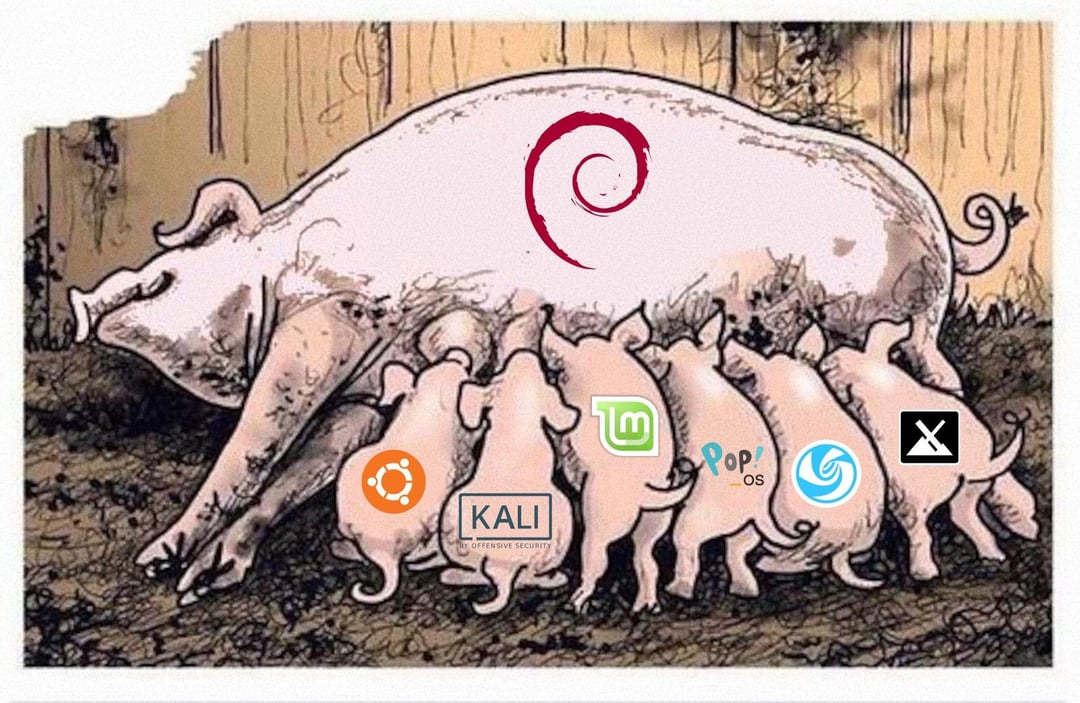
\includegraphics[width=0.70\textwidth]{images/forks.jpg}

\small \textbf{Потомки Debian}

\vspace{1cm}

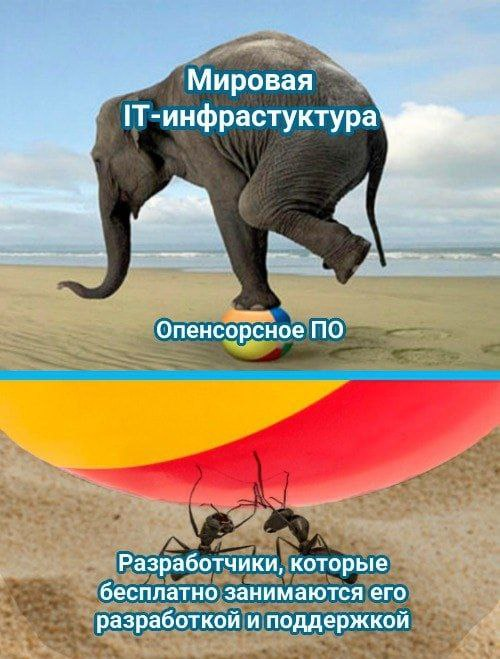
\includegraphics[width=0.70\textwidth]{images/motivation.jpg}

\small \textbf{Мотивация}
\end{center}


\vspace{-0.5cm}
\section*{1. Первые шаги в Debian}
\addcontentsline{toc}{section}{1. Первые шаги в Debian}
\vspace{-0.5cm}
\subsection*{\textbf{1.1 Salsa GitLab}}
\addcontentsline{toc}{subsection}{1.1 Salsa GitLab}
\vspace{-0.5cm}

Первым делом, можно зарегистрироваться в
\href{https://salsa.debian.org/public}{GitLab Salsa} --- это официальный
GitLab-сервер Debian. Там хранятся исходники пакетов, ведутся обсуждения,
принимаются merge request'ы и работает CI. Этот шаг углубит вас в мир Debian.

Можно и не регистрировать аккаунт, а придерживаться старого способа участия в
Debian, если вам так хочется:
\begin{itemize}
    \vspace{-0.3cm}
    \item отправлять патчи по email --- старый классический способ Debian;
    \item писать в BTS (bugs.debian.org);
    \item участвовать в обсуждениях.
    \vspace{-0.3cm}
\end{itemize}

Но если вы хотите участвовать в более современном формате, то лучше всё-таки
создать аккаунт в Salsa: так будет проще следить за репозиториями, отправлять
merge request'ы, участвовать в обсуждениях и пользоваться CI.

Пройдите регистрацию на \url{https://salsa.debian.org/users/sign_up}

\begin{center}
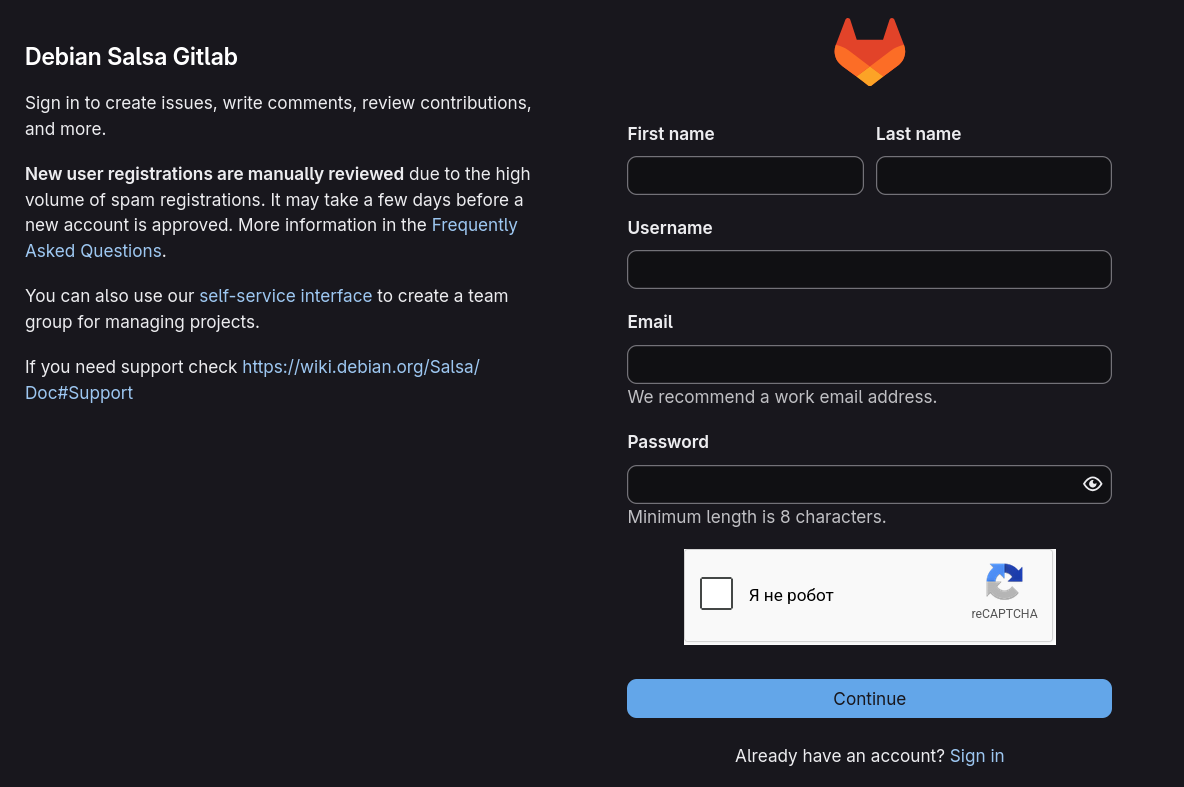
\includegraphics[width=0.70\textwidth]{images/salsa-sign-up.png}

\small \textbf{Salsa GitLab регистрация}
\vspace{-0.3cm}
\end{center}

и дождитесь, пока ваша учётная запись будет активирована (это может занять
некоторое время, наберитесь терпения).

\vspace{10cm}

После входа в аккаунт, можно добавить SSH-ключ \textbf{(Preferences ---> SSH
Keys)} --- он нужен, чтобы безопасно подключаться к GitLab и пушить/клонировать
репозитории без ввода пароля каждый раз.

\begin{center}
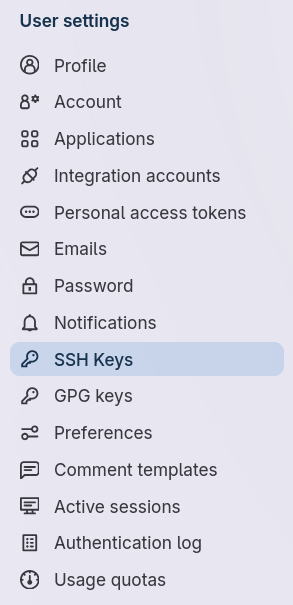
\includegraphics[width=0.20\textwidth]{images/salsa-ssh-keys.png}

\small \textbf{SSH Keys}
\vspace{-0.3cm}
\end{center}

Генерация SSH ключа происходит с помощью команды:
\vspace{-0.5cm}
\begin{verbatim}
$ ssh-keygen -f salsa
\end{verbatim}

\vspace{-0.3cm}
Скопируйте публичный ключ в буфер обмена:
\vspace{-0.5cm}
\begin{verbatim}
$ cat ~/.ssh/salsa.pub | xsel -b -i
\end{verbatim}

\vspace{-0.3cm}
Нажмите \textbf{Add new key} в GitLab и вставьте его в форму \textbf{Key}.

\textbf{Usage type: Authentication \& Signing}\\
(Authentication --- для входа/доступа по SSH)\\
(Signing --- для подписи Git-коммитов)

\textbf{Expiration date}: можете выбрать срок действия SSH-ключа. Если поставить дату,
ключ потом автоматически перестанет работать. Это полезно для безопасности. Я
обычно ставлю на 5 лет.

Удалите публичный ключ с вашего устройства:
\vspace{-0.5cm}
\begin{verbatim}
$ rm ~/.ssh/salsa.pub
\end{verbatim}

\vspace{-0.3cm}
Для безопасности проверьте, что у директории\texttt{~/.ssh} установлены права
\textbf{700}, а у приватного ключа\texttt{~/.ssh/salsa} --- \textbf{600}. Это
стандарт.

\vspace{10cm}

После того как вы настроили свой Salsa GitLab, можно немного осмотреться.

Ссылки:
\begin{itemize}
    \vspace{-0.3cm}
    \item \url{https://salsa.debian.org/public}
    \item \url{https://salsa.debian.org/explore/projects/starred}
    \vspace{-0.3cm}
\end{itemize}

\begin{center}
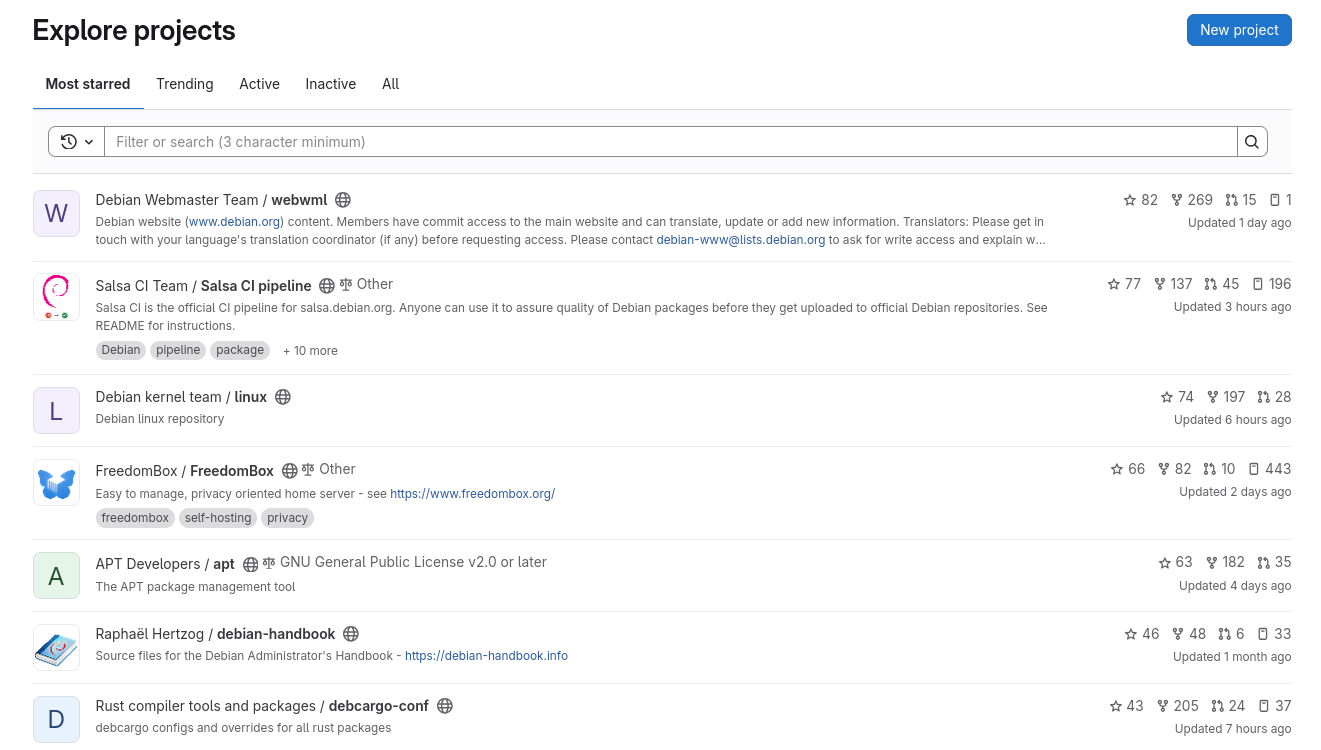
\includegraphics[width=0.95\textwidth]{images/salsa-view.png}

\small \textbf{Обзор Salsa GitLab}
\vspace{-0.3cm}
\end{center}

Думаю, вы уже заметили, что репозитории не просто разбросаны по GitLab, а
принадлежат определенным командам (Teams), которые регулярно обновляют
репозитории, исправляют баги, тестируют, делают какие-то правки и имеют
определенные привилегии в этих репозиториях. Вы можете посмотреть команды в
GitLab и увидеть, сколько репозиториев сопровождает каждая из них. Например,
если вас интересует ядро Linux в Debian, обратите внимание на
\url{https://salsa.debian.org/kernel-team}. Посмотрите на различные ветки в
репозиториях, на теги, коммиты, merge request'ы, CI и т.д.

Не пугайтесь, если чего-то не понимаете: это нормально. Сначала глаза
разбегаются, и может показаться, что всё слишком сложно, но со временем
структура репозиториев и рабочий процесс станут гораздо понятнее.

Тем более, многие инженеры в Debian работают не над всем сразу, а над
конкретными узкими задачами. Со временем перестаёшь замечать этот шум,
сосредотачиваешься на своей области, и всё становится гораздо проще. Нужно
просто занять свою нишу.

\vspace{10cm}

\subsection*{\textbf{1.2 Выбор направления и Debian Teams}}
\addcontentsline{toc}{subsection}{1.2 Выбор направления и Debian Teams}
\vspace{-0.5cm}

Давайте сначала разберёмся, как именно вы можете помочь Debian и куда можно
внести свой вклад.

Важная ссылка: \url{https://www.debian.org/intro/help.en.html}

Знайте: не все участники Debian являются разработчиками, и вам совершенно не
обязательно уметь программировать, чтобы участвовать. Есть множество способов
помочь Debian.

Если коротко, то:

1. Разработка и сопровождение пакетов.\\
   Писать программы, исправлять баги, делать патчи, сопровождать пакеты,
   заниматься безопасностью, портированием и инфраструктурой.

2. Тестирование и поиск ошибок.\\
   Проверять Debian и программы в нём, воспроизводить баги, отправлять отчёты в
   BTS, тестировать установщик и образы.

3. Документация.\\
   Писать инструкции, заметки, статьи, улучшать официальную документацию и
   Debian Wiki.

4. Переводы и локализация.\\
   Переводить программы, документацию, страницы сайта и проверять существующие
   переводы.

5. Помощь другим пользователям.\\
   Отвечать на вопросы, помогать на форумах, в Mailing Lists, IRC и других
   каналах общения.

6. Участие в мероприятиях.\\
   Помогать с DebConf, MiniDebConf, локальными встречами и другими событиями
   сообщества.

7. Пожертвования и ресурсы.\\
   Поддерживать Debian деньгами, железом, хостингом, зеркалами и другими
   ресурсами.

8. Популяризация Debian.\\
   Рассказывать о Debian, рекомендовать его другим, делать доклады, писать
   материалы, делиться опытом использования.

9. Поддержка от организаций.\\
   Компания или организация может помогать Debian ресурсами, спонсорством,
   инфраструктурой или рабочим временем сотрудников.

Задумайтесь, что вам нравится и что вам интересно в Debian. Может быть, есть
какой-то компонент, которым вы пользуетесь чаще других, и вам интересно, что в
нём происходит? Или у вас есть любимый текстовый редактор, терминал или
графическая оболочка? Может быть, вам интересны языки, и вы хотите вносить вклад
в локализацию любимых программ? Или вам хочется разбираться в CVE, тестировать
уязвимости и помогать с их исправлением? А может быть, вам интересны игры в
Debian? Или вам просто нравится главный сайт Debian, и вы хотите немного
подредактировать текст? Или вам нравится разбираться в конфигурации ядра и
улучшать её? А может, вам просто нравятся шрифты, иконки и всё такое? А может
CI? Контейнеризация? Виртуализация? Музыка/Видео? Браузер? Модули ядра?
Установщик Debian? Загрузка Debian? Перечислять можно бесконечно.

Начинать лучше с того, что вам уже нравится и чем вы сами пользуетесь: так
гораздо проще найти свою нишу, не потеряться в огромной экосистеме Debian и
постепенно превратить интерес в реальный вклад.

Например, я обожаю Vim и Xfce и использую их уже много лет. Соответственно, я
состою в Debian Vim Maintainers, делаю небольшой вклад и сопровождаю интересные
мне пакеты, а проекту Xfce по возможности помогаю через почтовую рассылку или
merge request'ы. Мне это интересно, потому что я сам активно этим пользуюсь.


\vspace{-0.5cm}
\section*{2. Подготовка рабочего окружения}
\addcontentsline{toc}{section}{2. Подготовка рабочего окружения}
\vspace{-0.5cm}
\subsection*{\textbf{2.1 Настройка репозиториев}}
\addcontentsline{toc}{subsection}{2.1 Настройка репозиториев}
\vspace{-0.5cm}

Репозиторий --- это сервер/хранилище, где хранятся пакеты для установки и
обновлений ОС (например, ядра, утилиты и программы). Он может содержать как
бинарные пакеты, так и исходные коды. Репозитории указываются в файле
конфигурации \texttt{/etc/apt/sources.list}. Существуют официальные репозитории
и сторонние, добавлять которые нужно с осторожностью, чтобы избежать
небезопасного ПО.

Бинарные пакеты --- это уже скомпилированные и готовые к установке программы или
утилиты.

Исходные коды --- это текстовые файлы, содержащие программу, которую нужно
скомпилировать в бинарный пакет перед установкой.

Как управлять \texttt{sources.list}: \url{https://wiki.debian.org/SourcesList}

Давайте рассмотрим мой \texttt{/etc/apt/sources.list} в качестве примера.

\begin{center}
\vspace{-0.3cm}
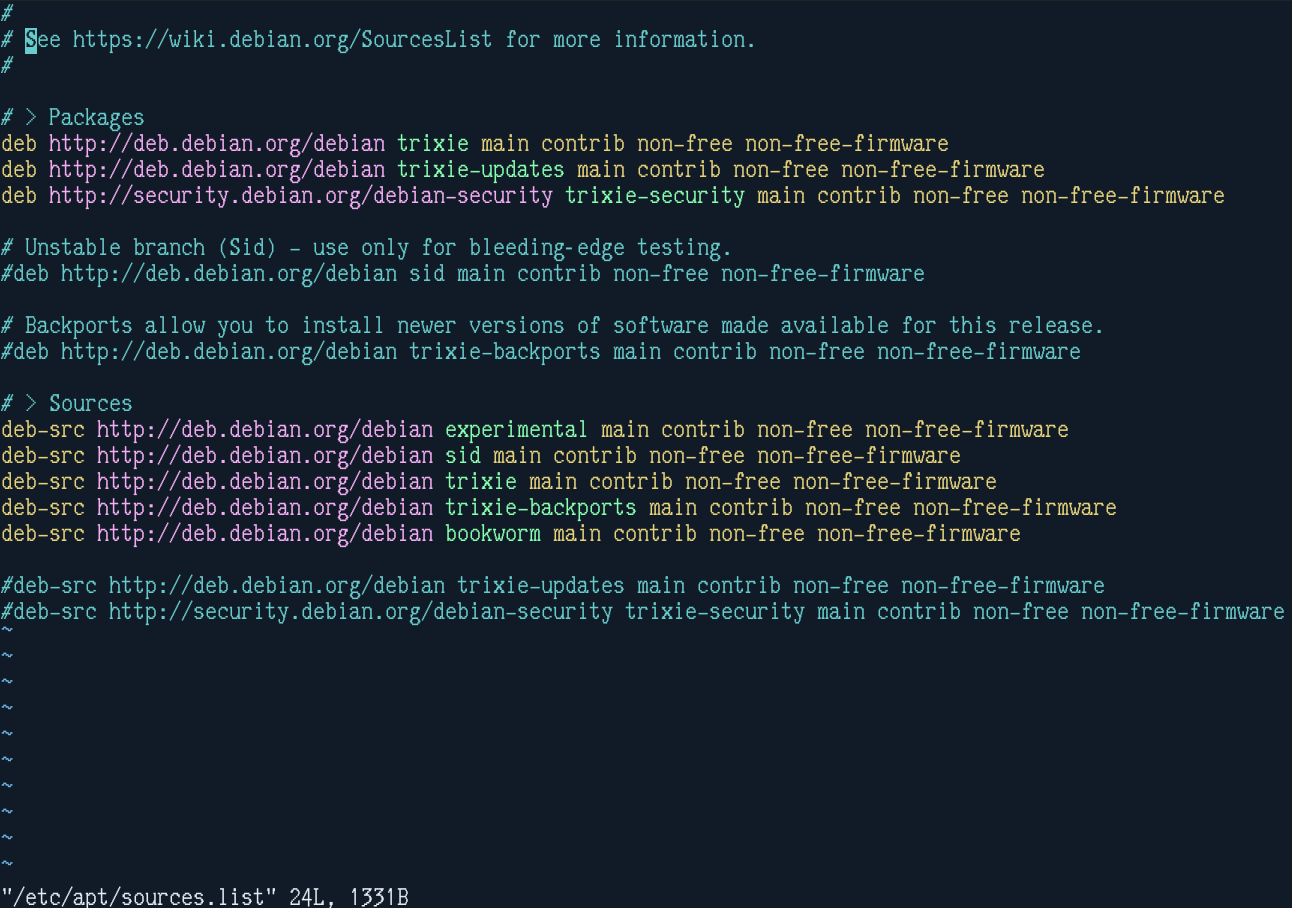
\includegraphics[width=0.95\textwidth]{images/sources-list.png}

\small \textbf{/etc/apt/sources.list}
\vspace{-0.3cm}
\end{center}

\vspace{10cm}

Структура:\\
\texttt{
deb http://site.example.com/debian distribution component1 component2\\
deb-src http://site.example.com/debian distribution component1 component2
}
\vspace{-0.5cm}

\textbf{deb}\\
бинарные пакеты

\textbf{deb-src}\\
пакеты с исходным кодом

\textbf{http://site.example.com/debian}\\
url репозитория

\textbf{distribution}\\
псевдоним релиза, ключевое слово, либо класс релиза

\textbf{component}\\
main, contrib, non-free, non-free-firmware набор пакетов

В секции бинарных пакетов у меня прописаны:\\
\textbf{trixie} основной репозиторий для стабильных пакетов Debian.
\textbf{trixie-updates} репозиторий для обновлений пакетов в основной версии,
включая исправления ошибок и улучшения. \textbf{trixie-security} репозиторий для
обновлений безопасности, содержит патчи и исправления уязвимостей.

В секции исходных пакетов у меня прописаны:\\
\textbf{experimental} содержит экспериментальные версии исходных пакетов,
которые используются для тестирования новых изменений. \textbf{sid} репозиторий
исходников нестабильной ветки Debian, где доступны самые свежие версии пакетов.
\textbf{trixie} исходные пакеты текущего стабильного релиза.
\textbf{trixie-backports} содержит исходники пакетов, перенесённых из более
новых веток для использования в \textbf{trixie}. \textbf{bookworm} исходные
пакеты предыдущего стабильного релиза, которые удобно использовать для сравнения
версий, изменений и сопровождения пакетов между выпусками.

Я прописываю столько секций \textbf{deb-src} только для одного: чтобы сравнивать
изменения и отслеживать их от релиза к релизу. Это нужно не всегда, но иногда
может понадобиться. Для начала работы с Debian достаточно указать свой релиз и
\textbf{sid} (так как мы будем работать с последними версиями пакетов).

\begin{center}
\vspace{-0.3cm}
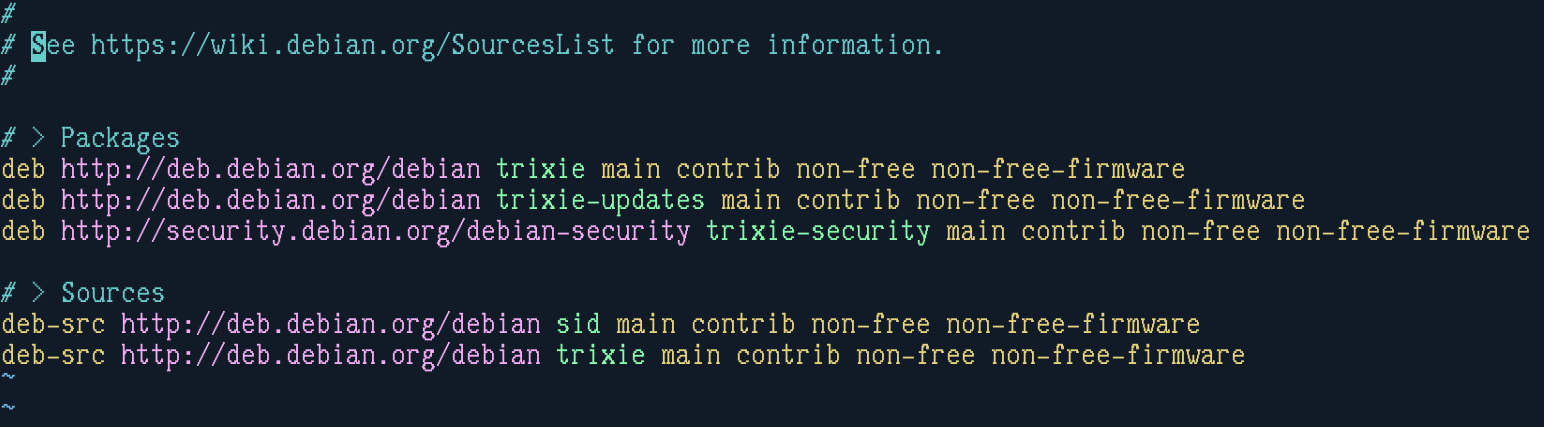
\includegraphics[width=0.95\textwidth]{images/sources-list-clean.png}

\small \textbf{/etc/apt/sources.list}
\vspace{-0.3cm}
\end{center}

\vspace{10cm}

Сделайте:
\vspace{-0.5cm}
\begin{verbatim}
$ apt-get update
\end{verbatim}

\vspace{-0.3cm}
Команда \texttt{apt-get update} обновляет локальный список пакетов, подтягивая
информацию о доступных пакетах и их версиях из репозиториев, указанных в
\texttt{/etc/apt/sources.list}.

После чего можно увидеть доступные версии исходного пакета для скачивания:
\vspace{-0.5cm}
\begin{verbatim}
$ apt-cache madison <package>
\end{verbatim}

\vspace{-0.3cm}
Например:
\vspace{-0.5cm}
\begin{verbatim}
$ apt-cache madison vifm
\end{verbatim}

\begin{center}
\vspace{-0.3cm}
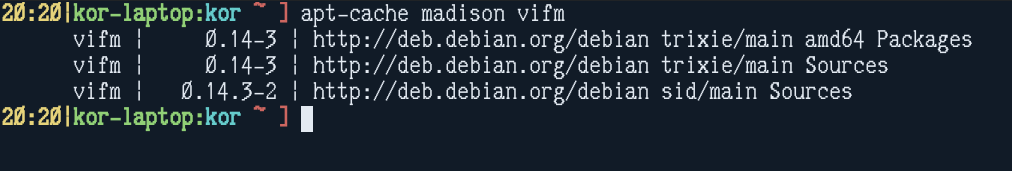
\includegraphics[width=0.95\textwidth]{images/madison-vifm.png}
\vspace{-0.5cm}
\end{center}

\vspace{-0.5cm}
\subsection*{\textbf{2.2 Инструменты и рабочая среда}}
\addcontentsline{toc}{subsection}{2.2 Инструменты и рабочая среда}
\vspace{-0.5cm}

Здесь описаны пакеты и инструменты, которые необходимо установить для базовой
работы с пакетами Debian.

\vspace{-0.5cm}
\begin{verbatim}
$ apt-get install build-essential dpkg-dev devscripts debhelper \
fakeroot lintian autoconf automake libtool dh-make dh-autoreconf \
quilt pbuilder
\end{verbatim}

\vspace{-0.3cm}
Это базовый набор инструментов, необходимый для сборки программ из исходного
кода, подготовки Debian-пакетов, проверки их качества и работы с типичным
autotools-проектом. С его помощью можно собрать программу, оформить её как
Debian-пакет, внести при необходимости патчи и проверить результат на
распространённые ошибки.

Также в список включён инструмент для сборки в чистом изолированном окружении
(pbuilder): он позволяет проверить, что пакет собирается только с указанными
зависимостями и не опирается на пакеты, случайно установленные в основной
системе.

Разработчики и мейнтейнеры Debian в основном собирают пакеты не на своей
основной машине, а в изолированной среде (chroot), чтобы не засорять рабочую
систему лишними зависимостями, устанавливаемыми для сборки, и при этом иметь
возможность проверить, что пакет действительно собирается только с теми
\texttt{Build-Depends}, которые явно указаны в его метаданных.

На практике для этого обычно используют \textbf{pbuilder} (хороший вариант для
начинающих) и \textbf{sbuild} (более распространённое решение для более
продвинутой и регулярной работы).

Важная ссылка: \url{https://wiki.debian.org/pbuilder}

\textbf{pbuilder} и \textbf{sbuild} по сути запускают \textbf{dpkg-buildpackage}
внутри чистого окружения (chroot), добавляя установку \texttt{Build-Depends} и
изоляцию. Это обертки над более низкоуровневыми инструментами.

Чтобы понять, из каких этапов состоит сборка, выполняемая
\textbf{dpkg-buildpackage}, можно обратиться к документации:
\url{https://man7.org/linux/man-pages/man1/dpkg-buildpackage.1.html}

Например, в Debian для автоматической сборки пакетов используется сеть
\textbf{buildd}-серверов. Исходные пакеты собираются в изолированных окружениях
с помощью \textbf{sbuild} и связанных с ним инструментов.

Сеть автоматической сборки: \url{https://www.debian.org/devel/buildd/}

Debian Package Auto-Building: \url{https://buildd.debian.org/}

Например, давайте посмотрим страницу \textbf{buildd} со статусом сборки пакета
vifm на разных архитектурах Debian:
\url{https://buildd.debian.org/status/package.php?p=vifm&suite=sid}

\vspace{-0.5cm}
\subsection*{\textbf{2.3 Структура исходного пакета}}
\addcontentsline{toc}{subsection}{2.3 Структура исходного пакета}
\vspace{-0.5cm}

Теперь мы готовы скачать исходный пакет
\href{https://tracker.debian.org/pkg/vifm}{vifm} и посмотреть его содержимое.
Обычно я перехожу во временную директорию \texttt{/tmp} и работаю там.
\vspace{-0.5cm}
\begin{verbatim}
$ apt-get source vifm # скачается самая последняя версия
\end{verbatim}

\vspace{-0.3cm}
Или скачать исходный пакет определенной версии:
\vspace{-0.5cm}
\begin{verbatim}
$ apt-get source vifm=0.14-3 # скачается версия из trixie
\end{verbatim}

\vspace{-0.3cm}
Исходный пакет будет скачан из репозитория Debian по адресу\\
\url{http://deb.debian.org/debian} (из соответствующей ветки/дистрибутива).


И так, мы имеем исходный пакет (source package):
\begin{center}
\vspace{-0.3cm}
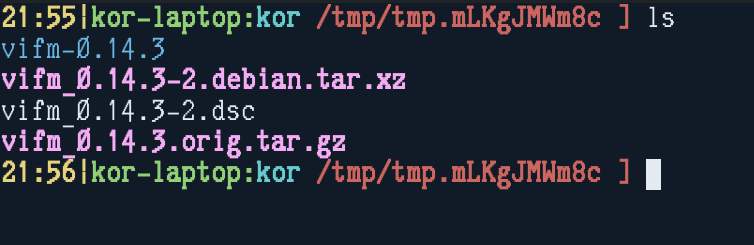
\includegraphics[width=0.95\textwidth]{images/source-package.png}
\end{center}

\vspace{10cm}

\textbf{vifm\_0.14.3.orig.tar.gz}\\
Оригинальные исходные файлы программы без изменений. Другими словами, это
неизмененные upstream-файлы от оригинальных авторов.

\textbf{vifm\_0.14.3-2.dsc}\\
Описание исходного пакета, где указана версия и ссылка на исходники. Этот файл
обычно подписывается сопровождающим пакета (подлинность).

\textbf{vifm\_0.14.3-2.debian.tar.xz}\\
Патчи и изменения для Debian (изменения в пакете, специфичные для Debian).

\textbf{vifm-0.14.3}\\
Директория, куда распаковываются файлы пакета.

Форматы файлов исходного пакета Debian могут различаться от пакета к пакету:
например, оригинальные исходные файлы и Debian-изменения могут быть упакованы в
архивы \textbf{.tar.gz}, \textbf{.tar.xz} или \textbf{.tar.bz2}, в зависимости
от выбранного способа сжатия. Поэтому набор файлов и их расширения не всегда
одинаковы, хотя их назначение остается тем же. Формат сжатия выбирает maintainer
пакета.

Давайте перейдем в директорию с исходными файлами пакета и посмотрим, что там:

\begin{center}
\vspace{-0.3cm}
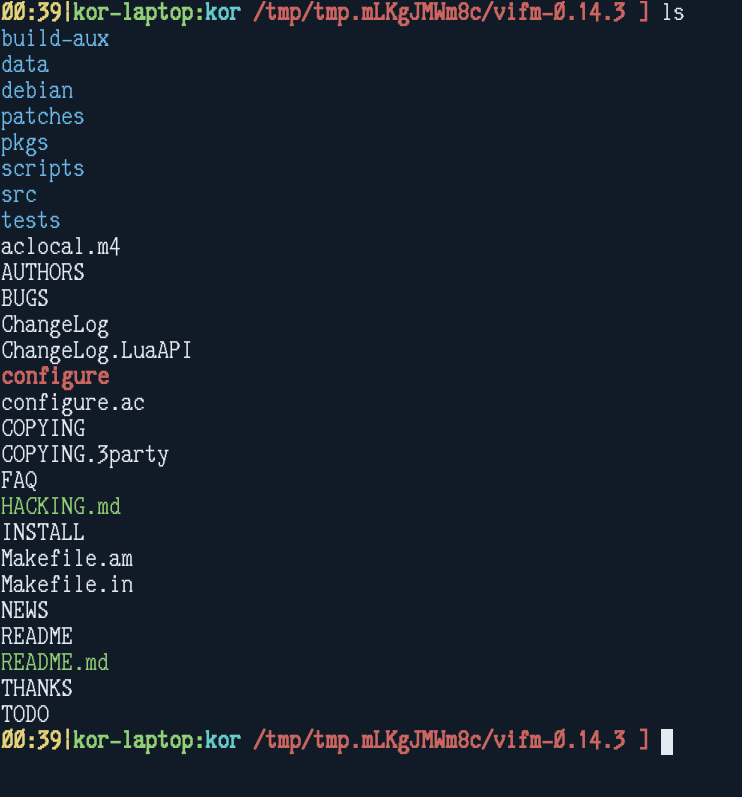
\includegraphics[width=0.70\textwidth]{images/source-files.png}
\end{center}

\vspace{10cm}

Если говорить просто, то перед нами исходное дерево проекта vifm. Сопровождающий
пакета взял исходные файлы из репозитория \url{https://github.com/vifm/vifm} и
импортировал их в Debian. На ранних этапах я бы не советовал слишком глубоко в
них погружаться, так как в структуре проекта легко потеряться.

Наличие файлов configure, configure.ac, Makefile.am, Makefile.in и aclocal.m4
показывает, что проект использует систему сборки Autotools. В дереве проекта
присутствуют исходный код, тесты, скрипты, данные и директория \textbf{debian/},
которая для нас наиболее важна.

Разработчики и мейнтейнеры Debian в основном работают с файлами в директории
\textbf{debian/}, где хранятся конфигурации для сборки пакета, патчи и другие
специфичные для Debian файлы. Им нужно гарантировать, чтобы программное
обеспечение успешно собиралось, правильно интегрировалось с системой и корректно
устанавливалось на всех поддерживаемых версиях Debian. Для этого они проверяют
совместимость, управляют зависимостями и обеспечивают соблюдение стандартов
качества, установленных для Debian-пакетов.

Я не буду здесь подробно останавливаться на назначении всех файлов, которые
могут встречаться в этой директории, поскольку для этого лучше обратиться к
руководствам из главы \textbf{Введение}, в частности к материалам
\textbf{среднего} уровня. Вместо этого предлагаю сосредоточиться на базовых
конфигурационных файлах на примере пакета
\href{https://tracker.debian.org/pkg/vifm}{vifm}.

\begin{center}
\vspace{-0.3cm}
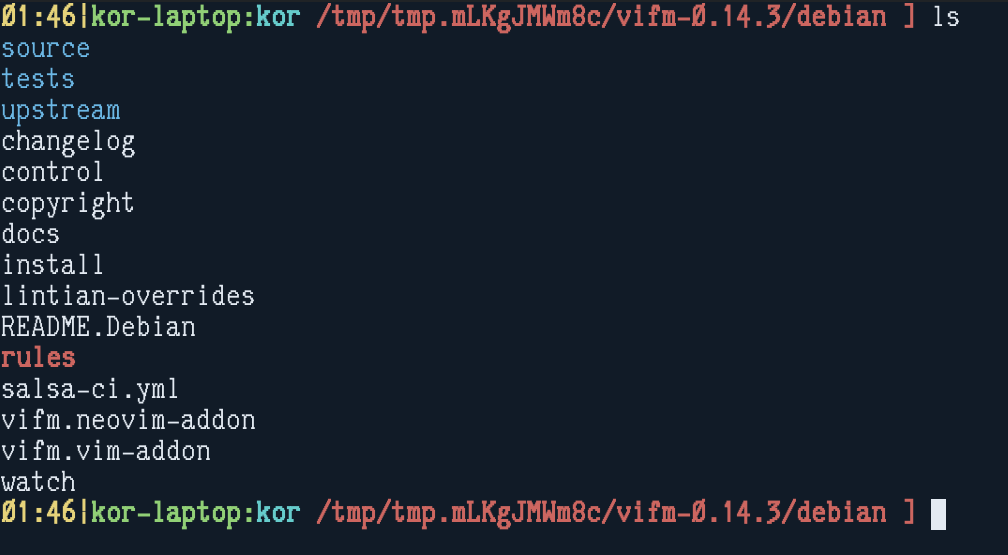
\includegraphics[width=0.95\textwidth]{images/debian-files.png}
\end{center}

\textbf{source}\\
Директория, содержащая дополнительные файлы, специфичные для сборки исходного
пакета.

\textbf{source/format}\\
Файл, указывающий формат исходного пакета, например, 3.0 (quilt).

\vspace{10cm}

\textbf{tests}\\
Директория с тестами, которые проверяют работоспособность пакета после установки
(autopkgtest).

\textbf{tests/control}\\
Конфигурационный файл для тестов, описывающий, какие тесты и как должны быть
выполнены.

\textbf{upstream}\\
Содержит информацию об исходных файлах проекта.

\textbf{upstream/metadata}\\
Upstream ссылки.

\textbf{changelog}\\
История изменений пакета с датами и описанием изменений в каждой версии.

\textbf{control}\\
Описание пакета, включая его название, описание, зависимости, версии и прочее.

\textbf{copyright}\\
Лицензионная информация о пакете, включая авторские права и условия
распространения.

\textbf{docs}\\
Директория с документацией, связанной с пакетом.

\textbf{install}\\
Файл, в котором перечисляют файлы и каталоги, которые нужно установить в пакет
при его сборке, а также куда именно их поместить.

\textbf{lintian-overrides}\\
Файл, в котором можно переопределить предупреждения и ошибки, генерируемые
инструментом
\href{https://manpages.debian.org/testing/lintian/lintian.1.en.html}{lintian}
при проверке пакета.

\textbf{README.Debian}\\
Документация, специфичная для Debian.

\textbf{rules}\\
Основной скрипт для сборки пакета, который описывает, какие команды и шаги нужно
выполнить для компиляции и упаковки пакета. Тут пригодятся знания Makefile.

\textbf{salsa-ci.yml}\\
Конфигурация для CI/CD (непрерывной интеграции), специфичная для платформы Salsa
(GitLab Debian). Можно посмотреть, как это работает на практике
\url{https://salsa.debian.org/debian/vifm/-/pipelines}

\textbf{watch}\\
Файл, который указывает, где можно отслеживать обновления исходного кода пакета.
Чаще всего это GitHub.

Подробно изучите каждый файл, особенно \textbf{control} и \textbf{rules}. Если
вас интересует, что значит каждое поле в \textbf{control}, можно полистать
\url{https://www.debian.org/doc/debian-policy/ch-controlfields.html}.

Структура пакетов Debian в целом единообразна, поэтому при работе с ними быстро
привыкаешь к принятым стандартам. В Debian большое значение придаётся правилам
оформления пакетов. Их соблюдение обеспечивает аккуратную структуру пакета,
корректную интеграцию в систему, а также совместимость, удобство установки и
последующего обновления. Поэтому желательно знать
\href{https://www.debian.org/doc/debian-policy/}{Debian Policy} --- не целиком,
но хотя бы в основных моментах.


\end{document}
